%!TEX root=document.tex

\section{Qualitative Study}\label{sec:example-viz}

In this section, we study some examples of visualizations recommended and
not recommended by \SeeDB for real-world datasets.
We turn to the BANK and DIAB dataset described in 
Section~\ref{sec:experiments}.
 
We begin with the DIAB dataset. The query selects a group of diabetes patients in the age range 30--40;
these patients are compared against all patients.
In Figure~\ref{fig:qual-study}, we list one example of a visualization
that is recommended by \SeeDB, and one that is not recommended by \SeeDB.
We acknowledge that the charts outputted by \SeeDB could look prettier and be better
formatted to make the output more usable and interpretable; this has not been our focus thus far. 
We plan to address these presentation issues in the future.

The visualization recommended by \SeeDB (Figure~\ref{fig:time-in-hospital}) has utility 0.174 (via
the Earth Mover's Distance utility metric).
This visualization depicts the time in hospitals spent by
individuals of different race, for the selected patients
(i.e., those between 30 and 40), and
the rest. 
As can be seen in this figure, this visualization is indeed interesting;
when we compare the average amount of time spent in hospital 
for african americans and caucasians, 
for the selected patients, the amount of time spent in hospital
by african americans and caucasians is quite close to each other,
while across all age groups, caucasians spend a lot more time
in hospital.

The visualization not recommended by \SeeDB (Figure~\ref{fig:lab-procedures}) has utility 0.004, very close to 0.
This visualization depicts the fraction of patients that 
have either had or not had lab procedures. 
As can be seen in the figure, the same fraction of patients in
both the selected patients as well as all patients
have had lab procedures.
This is therefore not as interesting a visualization.

Next, we consider the BANK dataset. 
Here the query selects all divorced individuals, 
and these are compared against all individuals. 
In Figure~\ref{fig:qual-study2}, we depict
a visualization recommended and one that is not recommended by \SeeDB.
The one recommended (Figure~\ref{fig:job}) depicts the fraction of calls made in the previous campaign (hence the y-axis is denoted previous) to those
who are divorced and had different job categories.
For instance, the number of retired divorced individuals who were called
is much higher than those that were blue caller divorced individuals,
while the opposite is true in general.
Perhaps this is an indication that the bank should target more blue caller divorced
individuals in the next campaign.
Thus, this is an interesting visualization.

On the other hand, the one not recommended (Figure~\ref{fig:loan})
depicts the fraction of calls made in the current campaign to those
whose loan status is either yes, no or unknown. 
Here the distribution is similar for divorced individuals and the rest.
Thus, this is not as interesting a visualization.

As can be seen, 
the visualizations produced by \SeeDB based on the Earth Mover's Distance
metric ends up giving useful, interesting visualizations on two of
the real world datasets we have experimented with.



\begin{figure}[h] 
\centering
\begin{subfigure}{\linewidth}
\centering
{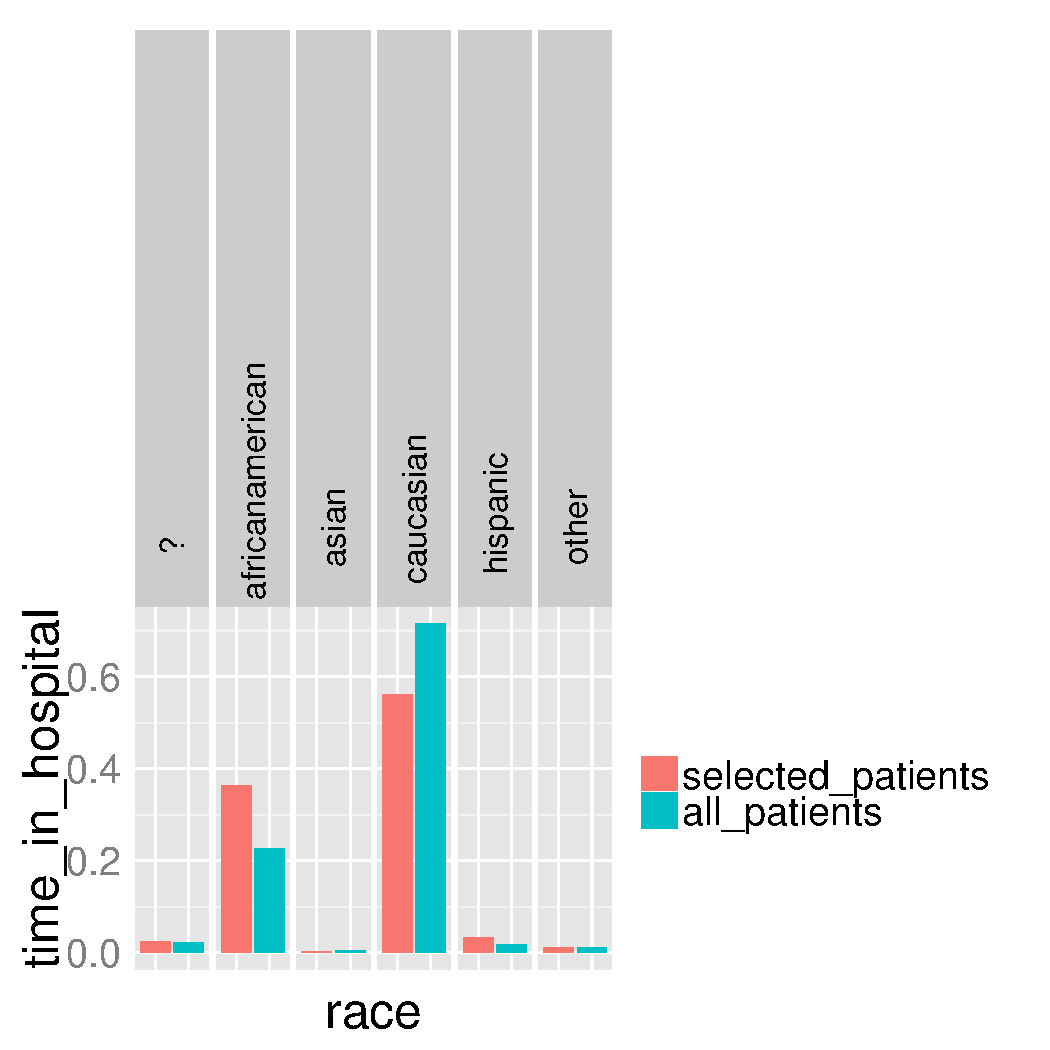
\includegraphics[width=7cm] {Images/seedb_dim_race_measure_time_in_hospital.pdf}}
\caption{Time in Hospital by Race: Recommended by \SeeDB}
\label{fig:time-in-hospital}
\end{subfigure}
\begin{subfigure}{\linewidth}
\centering
{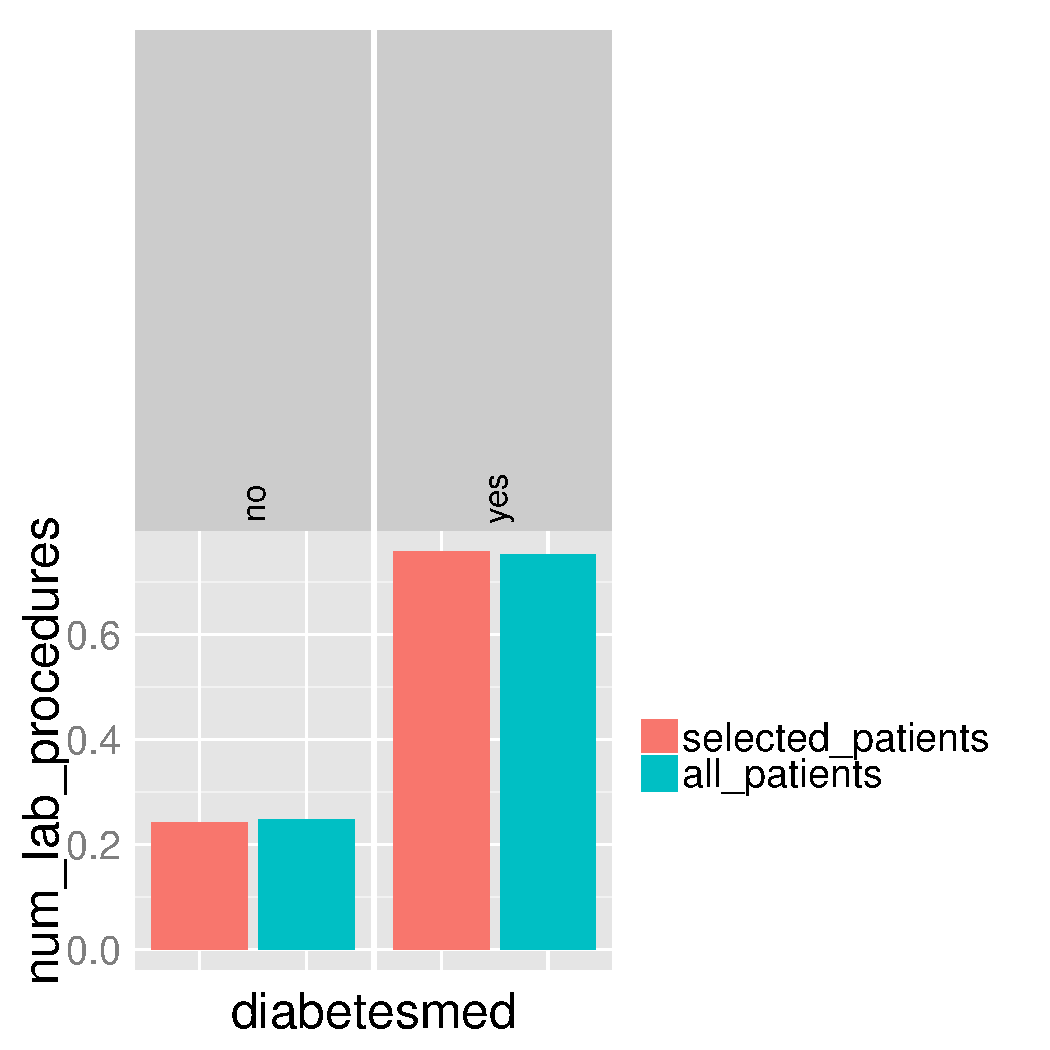
\includegraphics[width=7cm] {Images/seedb_dim_diabetesmed_measure_num_lab_procedures.pdf}}
\caption{Lab Procedures: Not Recommended by \SeeDB}
\label{fig:lab-procedures}
\end{subfigure}
\vspace{-10pt}
\caption{\SeeDB Generated Visualizations for DIAB}\label{fig:qual-study}
\vspace{-10pt}
\end{figure}


\begin{figure}[h] 
\centering
\begin{subfigure}{\linewidth}
\centering
{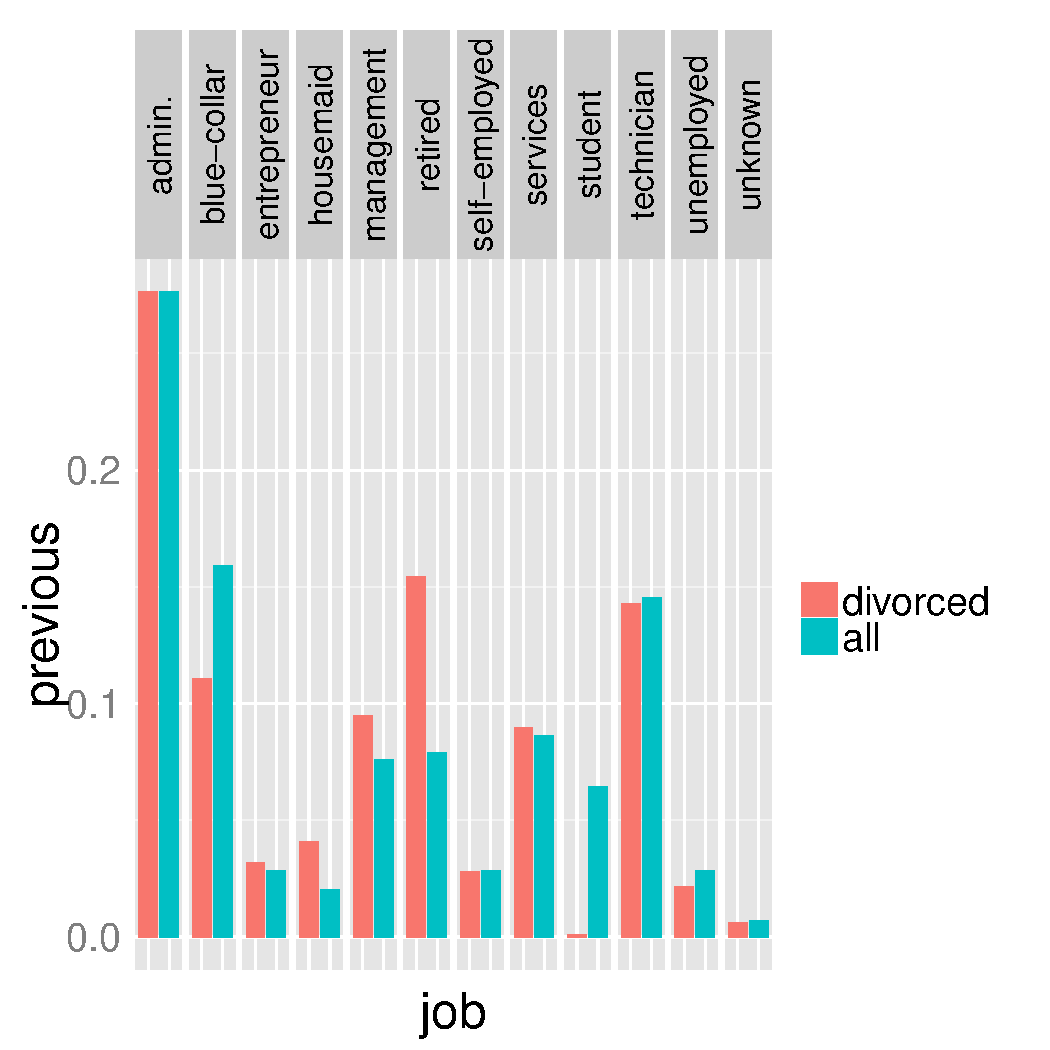
\includegraphics[width=7cm] {Images/seedb_dim_job_measure_previous.pdf}}
\caption{Fraction of calls made to different job holders: Recommended by \SeeDB}
\label{fig:job}
\end{subfigure}
\begin{subfigure}{\linewidth}
\centering
{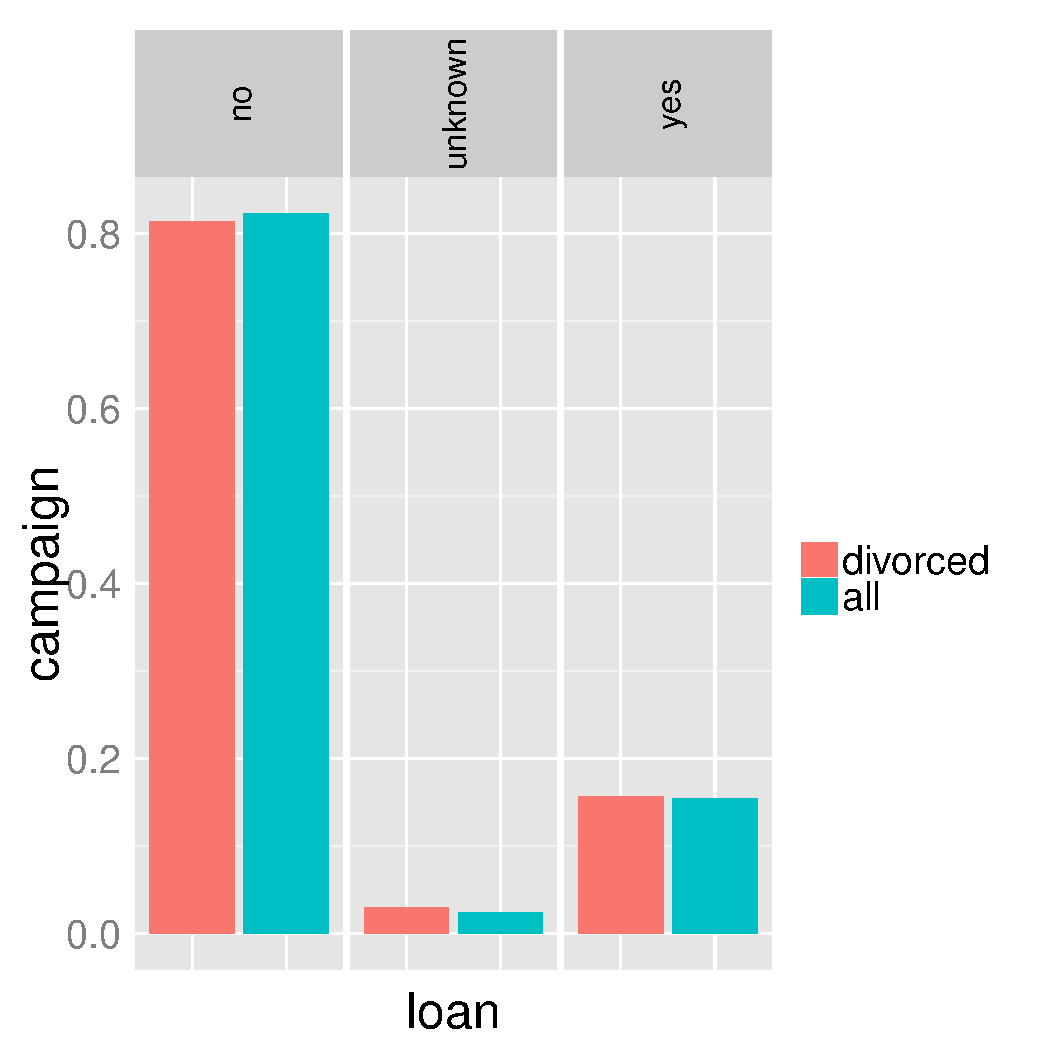
\includegraphics[width=7cm] {Images/seedb_dim_loan_measure_campaign.pdf}}
\caption{Fraction of calls made to those with different loan approval status: Not Recommended by \SeeDB}
\label{fig:loan}
\end{subfigure}
\vspace{-10pt}
\caption{\SeeDB Generated Visualizations for BANK}\label{fig:qual-study2}

\vspace{-10pt}
\end{figure}